
\documentclass[a4paper]{article}
\usepackage[spanish]{babel}
\selectlanguage{spanish}
\usepackage[utf8]{inputenc}
\usepackage[T1]{fontenc}
\usepackage{graphicx}


\title{Mi aprendizaje en  \LaTeX}
\author{Paula Córdoba Peláez\\
  \small Universidad de Granada\\
  \date{Diciembre 2020}
}
\usepackage{float}
\begin{document}
\maketitle
\newpage
\begin{abstract}
Este es el proyecto final del curso de \LaTeX que he realizado.  Me ha resultado muy interesante aprender a manejar esta plataforma, y creo que será de utilidad en el futuro. También he aprendido a utilizar Git,  otra herramienta muy interesante.
$ Url: https://github.com/paucorx/proyecto\_final $
\section{Introducción}
En este curso he realizado distintas actividades como creación de tablas,  imágenes y demás en esta aplicación. También he aprendido a crear repositorios en Git y a sincronizarlo con Git Hub.
\subsection{Lo que sé hacer con \LaTeX}

Insertar tablas:\\
\begin{table}

\end{table}
\begin{table}[H]
\centering
\begin{tabular}{l c r} 
l para left & c para centro & r para derecha \\ \hline
Ejemplo & Centrado & Alineado a la\\
Izquierda & 13 & Derecha
\end{tabular}
\caption{\label{tab:tabla ejemplo}Una simple tabla.}
\end{table}
\newpage
Insertar imágenes: \\
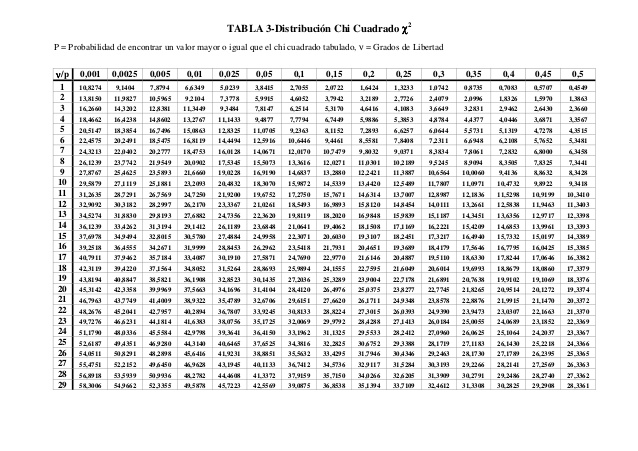
\includegraphics[scale=0.5]{tabl} \\
Insertar fórmulas: \\
\begin{equation}
e^{i\pi} + 1 = 0
\end{equation}
$ \sin^2 x + \cos^2 x = 1 $
\end{abstract}
\newpage
\bibliography{trabajo}
\bibliographystyle{plain}
\cite{Latex}
\cite{Zaikov:aa}
\cite{Mabey:1991aa}
\cite{Markovic:aa}

\end{document}
